\chapter{Article 3 - Evolutionary mechanisms driving the loss of the intromittent phallus in avian lineages}
\label{IPLOSS}

\begin{center}
    \large Alexandre Laverré$^{\text{1}}$, Maëva Luxey$^{\text{1}}$, Patrick Tschopp$^{\text{2}}$, Anamaria Necsulea$^{\text{1}}$\\
    \vspace{0.5cm}
    \normalsize
    $^{\text{1}}$Univ Lyon, Université Claude Bernard Lyon 1, CNRS, Laboratoire de Biométrie et Biologie Evolutive, F-69100, Villeurbanne, France.\\
    $^{\text{2}}$Laboratory of Regulatory Evolution, DUW Zoology, University of Basel, Basel CH-4051, Switzerland\\
\end{center}

{\hypersetup{linkcolor=GREYDARK}\minitoc}

\section{Abstract}

\section{Introduction}

The vertebrates’ transition from aquatic environments to life on land, more than 300 million years ago, was accompanied by multiple morphological and physiological adaptations, among which internal egg fertilization represented an important reproductive advantage. This mode of reproduction is evidently facilitated by the presence of an intromittent phallus (IP), which helps sperm delivery to the egg. However, although an intromittent male reproductive organ was likely present in the amniote ancestor, it was reduced or entirely lost in multiple avian lineages (Herrera et al. 2013). The evolutionary processes that led to phallus reduction or loss in these species, which nevertheless retained internal fertilization are still unclear. Given that mating with males lacking an IP requires female cooperation and thus allows females more control over fertilization, one hypothesis posits that this process occurred as a result of sexual selection through female choice of mates (Briskie & Montgomerie, 1997). It was also proposed that IP loss was a consequence of natural selection, as it reduced the risk of sexually transmitted diseases, which is elevated in species with a common passage for the urogenital and gastrointestinal systems (Briskie & Montgomerie, 1997). The developmental processes and molecular mechanisms that are responsible for phallus reduction or loss are also not fully understood. It was shown that, in the chicken, this process occurs through an activation of cell death  signals  in  the  developing  genitals,  caused  by  a  gain  of  expression  in  an  important  developmental  factor (Herrera et al., 2013). The genetic basis of this evolutionary change in gene expression is yet unknown. The molecular underpinnings of this morphological transformation are further complicated by the fact that the genes involved in IP development are highly pleiotropic, functioning for example in limb development (ref?). Moreover, many of the regulatory elements that control developmental gene expression are shared between limbs and genitalia (ref). A non-adaptive mechanism for IP reduction/loss can thus be envisaged, as a side-effect of evolutionary changes in other anatomical structures with shared developmental mechanisms (ref).\\

The main aim of this study is to understand the evolutionary processes and molecular mechanisms that drive the loss of the intromittent phallus in avian lineages. The recent publication of numerous avian genome sequences (6), as well as the increasing accessibility of technologies that assay gene expression and regulation, offers an opportunity to address these questions at an unprecedented scale. Through comparative analyses, we propose to evaluate selective pressures associated with IP loss in avian lineages at a genome-wide level, thus revealing the developmental genes and regulatory elements involved in this major morphological transformation. We assessed selective pressures acting at two different genomic levels. \\

- gene expression evolution between chicken and duck
- regulatory sequence activity and evolution between samples
- sequence evolution in birds lineages

We tested the presence  of  selection  on  non-coding  regulatory  elements,  expected  if  changes  in  gene  expression  patterns  (rather than in gene products) are at the origin of the loss of the IP. The existence of multiple independent events of IP reduction/loss during avian evolution, which highlights the remarkable selective pressures that act on this organ, is a key point in our proposal. Our comparative analyses can predict genes and regulatory elements that have exclusive roles in IP development in the avian ancestor, as these elements are expected to evolve rapidly in all IP-lacking lineages, following the loss of functional constraints. \\

\section{Results}

\subsection{Gene expression differences during the development of phallus precursors in chicken and duck}

\begin{figure}[h]
    \centering
    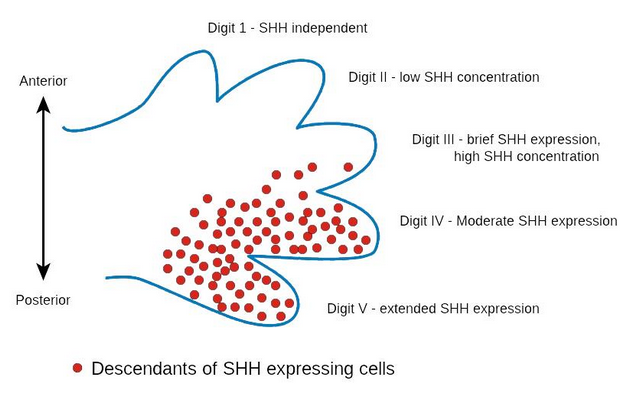
\includegraphics[width=1\textwidth, page=1] {figures/IPLOSS/fig1.png}
    \caption[Gene expression differences.]{
    \textbf{Gene expression differences.}\\
    }
    \label{fig:IPLOSS-fig1}
\end{figure} 

\begin{figure}[h]
    \centering
    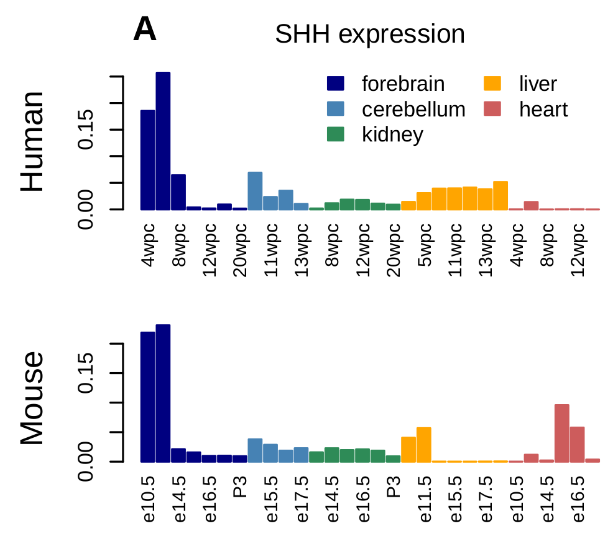
\includegraphics[width=1\textwidth, page=1] {figures/IPLOSS/fig2.png}
    \caption[Clusters of temporal gene expression.]{
    \textbf{Clusters of temporal gene expression.}\\
    }
    \label{fig:IPLOSS-fig2}
\end{figure} 


\subsection{Regulatory sequences that control phallus development in chicken and duck}

To determine the regulatory elements that control gene expression during chicken and duck external genitalia development, we analyzed open chromatin regions with the ATAC-seq technique at embryonic stages 29 and 33 (ref). At stage 29, the GT grows in both species, whereas at stage 33 the chicken GT begins to degenerate (ref). In order to identify GT-specific regulatory regions we analysed previously published ATAC-seq data for several organs in both species (ref). The number of open chromatin regions (ATAC-peak) is heterogeneous between samples (Figure 2.A). Chicken GT samples show a surprisingly low number of ATAC-peaks (35,725 and 38,394 for GT 29 and 33) compared to other samples. The number of non-GT duck ATAC-peaks are about two fold higher than other samples (test, pval). \\

- transcription factors binding site enrichment GT vs other (Methods)

The proportions of exonic, intronic and intergenic regions are not significantly different between samples. The number of ATAC-peaks detected in samples are correlated to the sequencing depth (Supplementary Figure, correl test, pval). In order to compare the open chromatin regions between samples without this evident bias, we drew the same number of ATAC-peaks for each sample within species (Methods). We identified ATAC-peaks homologous regions between species from a whole-genome alignment (Methods). The proportion of homologous regions identified did not differ between samples (Supplementary Fig). However, the average identity score is significantly lower for chicken GT ATAC-peaks at stage 29 (Figure 2.B). For each homologous region we determined whether it also covered an ATAC-peak of the other species (Methods). Based on these homologous activities, the factorial correspondence analysis separates the samples by species (Figure 2.C). The chicken GT ATAC-peaks are closest to those obtained in cells of lower and upper limb development. This appears to be consistent with the large number of cis-regulatory regions shared during the development of these organs during development in mouse (ref). Duck genital tubercle ATAC-peaks are most similar to those of the chicken. More than 20\% of the duck GT ATAC-peaks are also active in the chicken GT (Figure 2.D). Less than 15\% of the duck non-GT ATAC-peaks are observed in any of the chicken samples.

\begin{figure}[h]
    \centering
    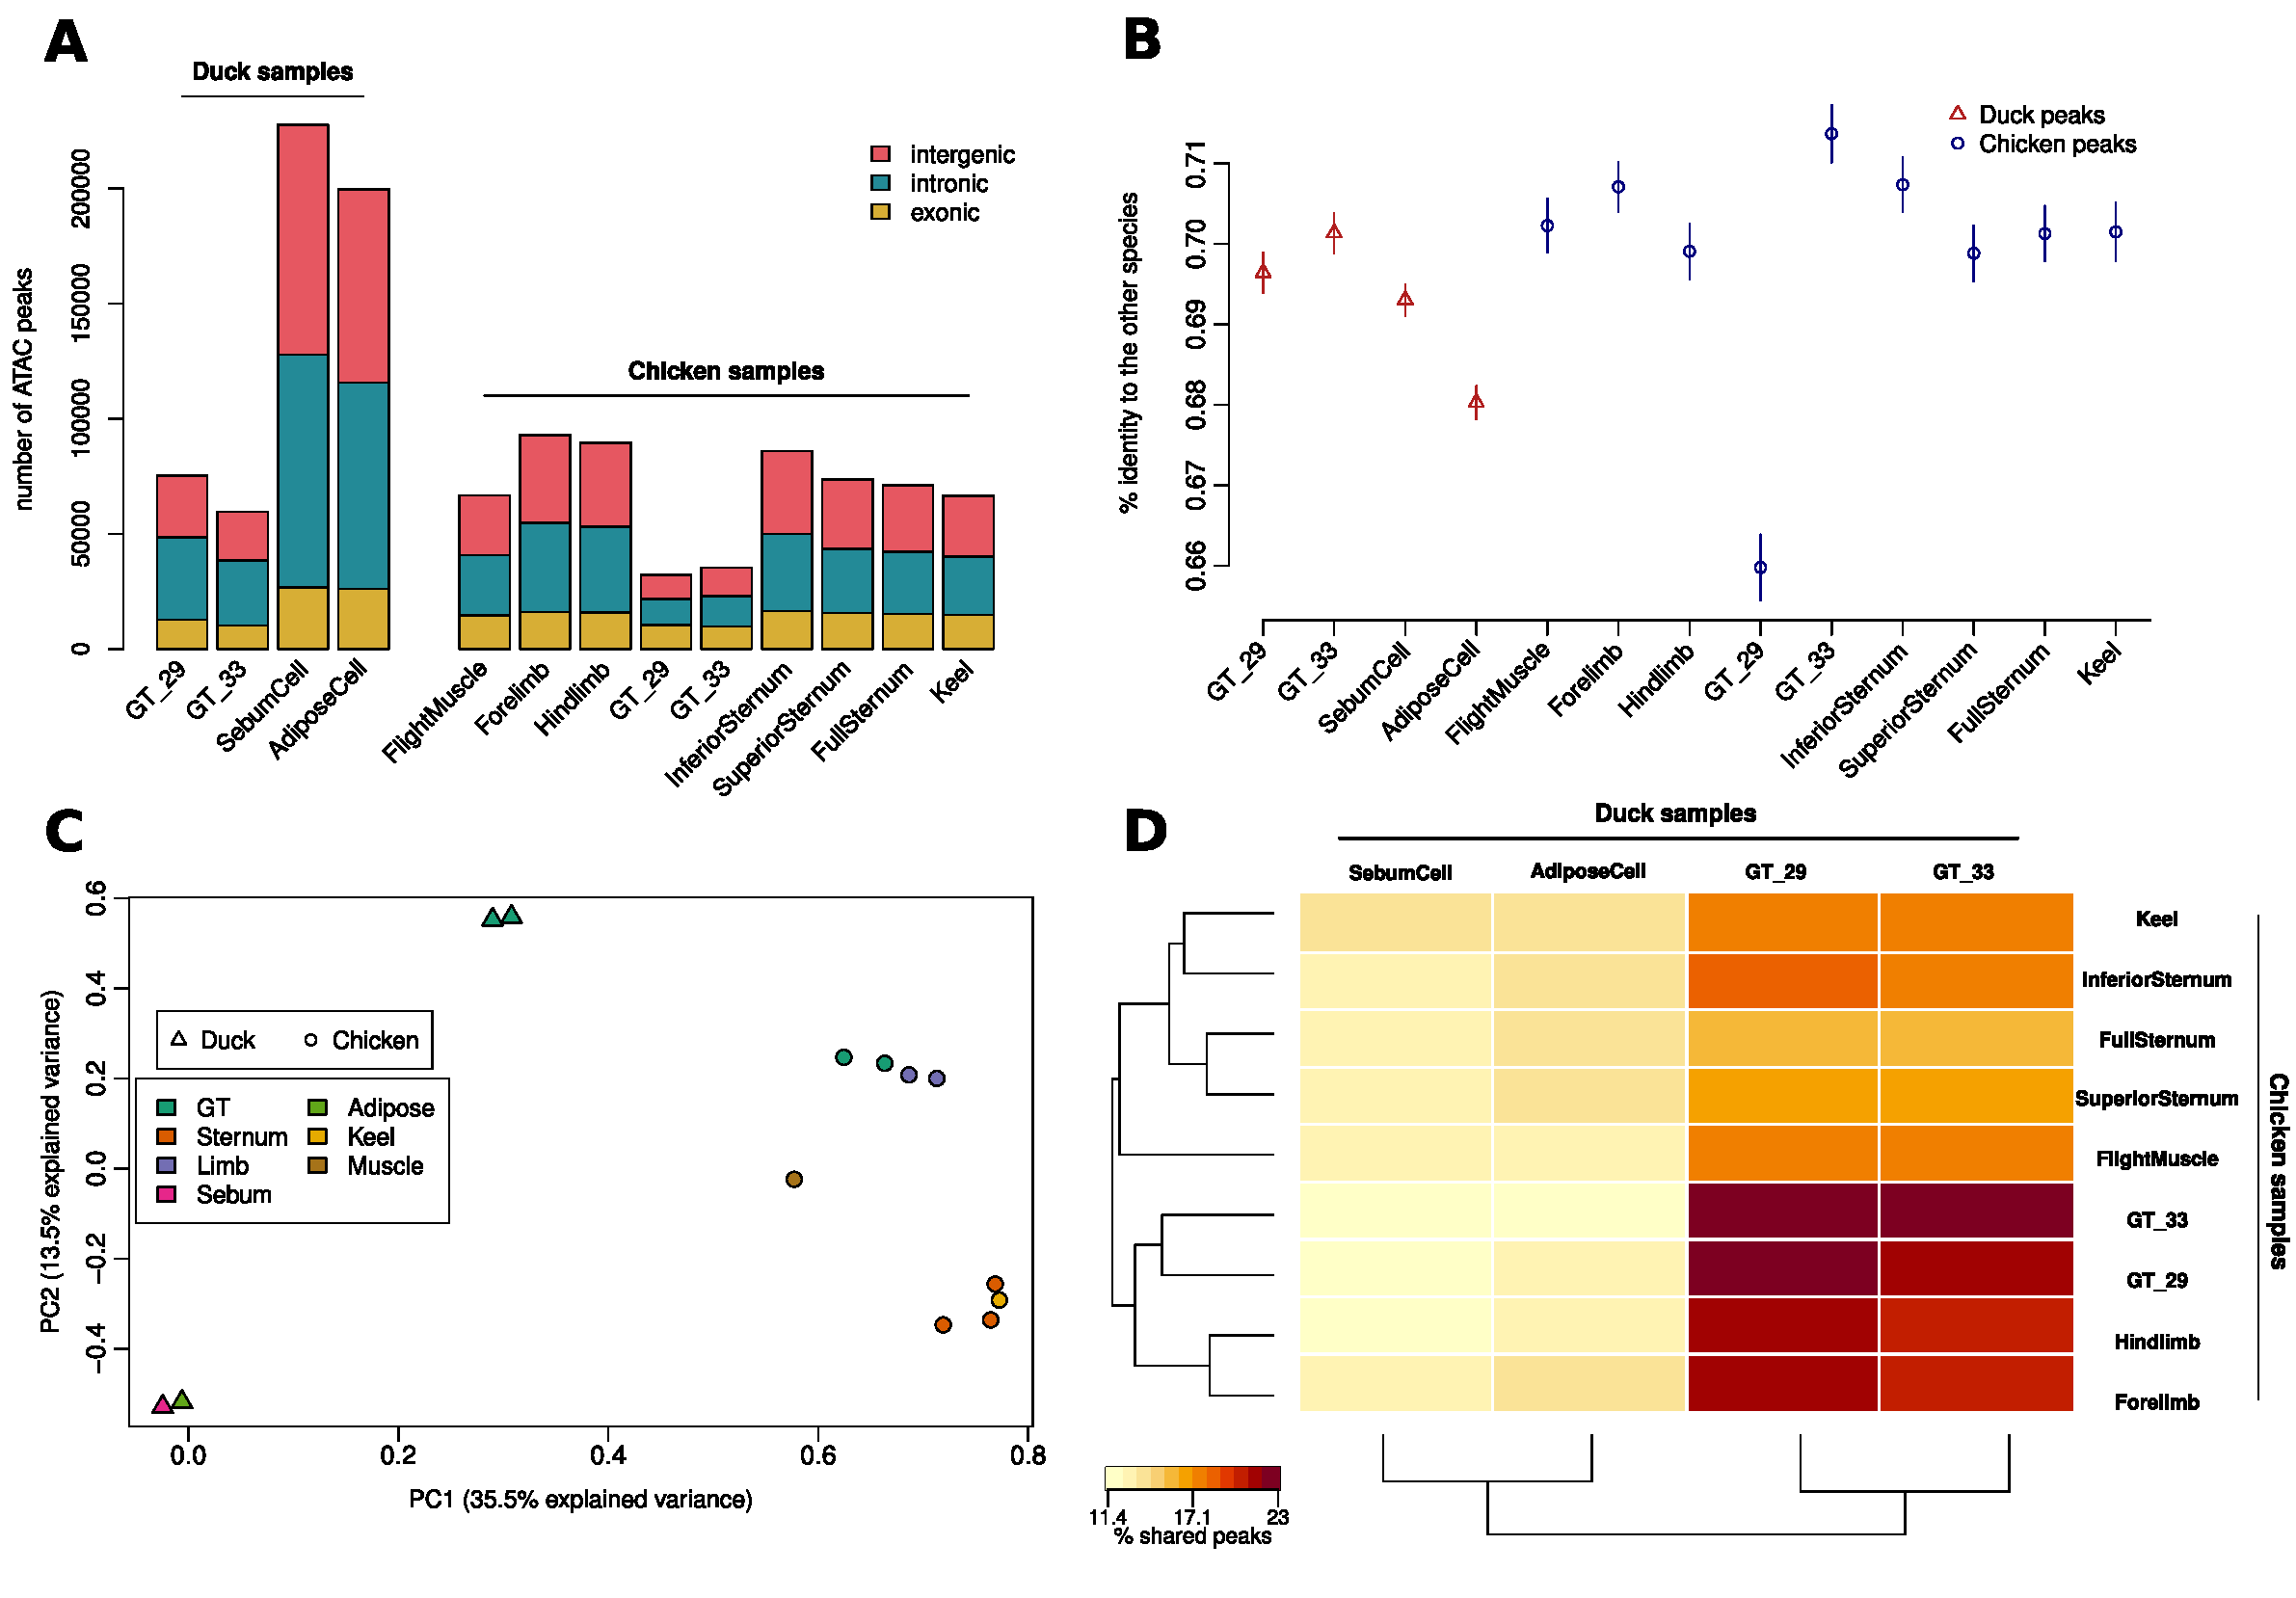
\includegraphics[width=1\textwidth, page=1] {figures/IPLOSS/Fig_peaks.pdf}
    \caption[Comparison of ATAC data in duck and chicken samples.]{
    \textbf{Comparison of ATAC data in duck and chicken samples.}
    \textbf{A.} Distribution of the number of ATAC peaks detected in duck and chicken samples. Peaks are classified according to their overlap with at least one exonic base (exonic, yellow), one non-exonic base (intronic, blue) or no genic base (intergenic, red). 
    \textbf{B.} Distribution of the median percentage identity between sub-sampled duck ATAC peaks sequences (N=63,250) aligned in the chicken genome (red triangle), and between sub-sampled chicken ATAC peaks sequences (N=35,725) aligned in the duck genome (blue circle). Error bars represent the 95\% confidence interval of median. 
    \textbf{C.} Principal component analysis of chicken and duck samples based on homologous subsampled peak activity. Homologous sequences of peaks from a reference species are active in the target species if they overlap at least one base of an ATAC peak in this species (Methods). \textbf{D.} Proportion of subsampled duck ATAC peaks whose homologous sequence overlaps with an ATAC peak in the chicken samples. Dendrograms are produced from the ATAC peak activity binary matrix of each species.  \\
    }
    \label{fig:IPLOSS-fig3}
\end{figure} 

\subsection{Regulatory sequences evolution in bird lineages}
Regulatory elements that control gene expression in the intromittent phallus (IP) are expected to display accelerated evolution in the lineages where this organ was lost, due to relaxation of purifying selection. Evolutionary sequence analyses can thus help identify elements that function in this organ. We analysed the sequence evolution of all non-exonic ATAC peaks detected in duck (N=X) and chicken (N=Y) samples within the aligned genomes of 53 bird species (Figure 3.A; Methods). Of these species, 21 possess an IP and the phylogenetic distribution of this phenotype would represent 5 independent convergent losses (ref). We also complemented this analysis with the identification of non-coding sequences from another duck species (Cairina moschata) conserved in all birds with an IP (Methods). \\

For each aligned sequence, we estimated relative evolutionary rates within each lineage (Methods). A high relative evolution rate in a lineage indicates an accelerated divergence of the sequence relatively to all analysed sequences in that lineage. For each alignment, we estimated the correlation between the relative evolutionary rates and the phenotypic distribution of the IP along the phylogeny (Figure 3.B; Methods). A positive correlation coefficient indicates that the sequence underwent a convergent acceleration of its evolutionary rate in species that lost IP. Conversely, a negative correlation coefficient indicates that lower relative rates of evolution are associated with species that have an IP. The most correlated duck ATAC peak has a median relative evolutionary rate of X in species with IP and Y in species without (Rho = ; FDR=). The proportion of sequences significantly associated with the presence of IP is low for all samples (Figure 3.C; median Duck samples = Y; Supplementary Figure Chicken & Cairina). For duck ATAC peaks, there is a convergently accelerated sequence enrichment in species without IP (test; pval). There is also a higher proportion of sequence correlated with IP evolution in GT samples than in other tissues (test; pval). To assess the impact of the distribution of IP along phylogeny on the correlation with relative evolutionary rates, we performed random permutations of the presence of IP across lineages (Figure 3.D). The median of the observed absolute correlation coefficients is significantly higher than the random permutations (pval=Z). Furthermore, the average number of ATAC peaks correlated with the presence of IP in the random permutations is significantly lower than that observed for the distribution of true phenotypes (obs=1300; random perm.=Y; pval=Z; Supplementary Figure). We detected 535f sequences significantly correlated with the IP evolution and detected by ATAC-seq in duck GT samples. A small proportion of them overlap the chicken ATAC peaks and the conserved Cairina sequences among IP birds (Figure 3.E).

\begin{figure}[h]
    \centering
    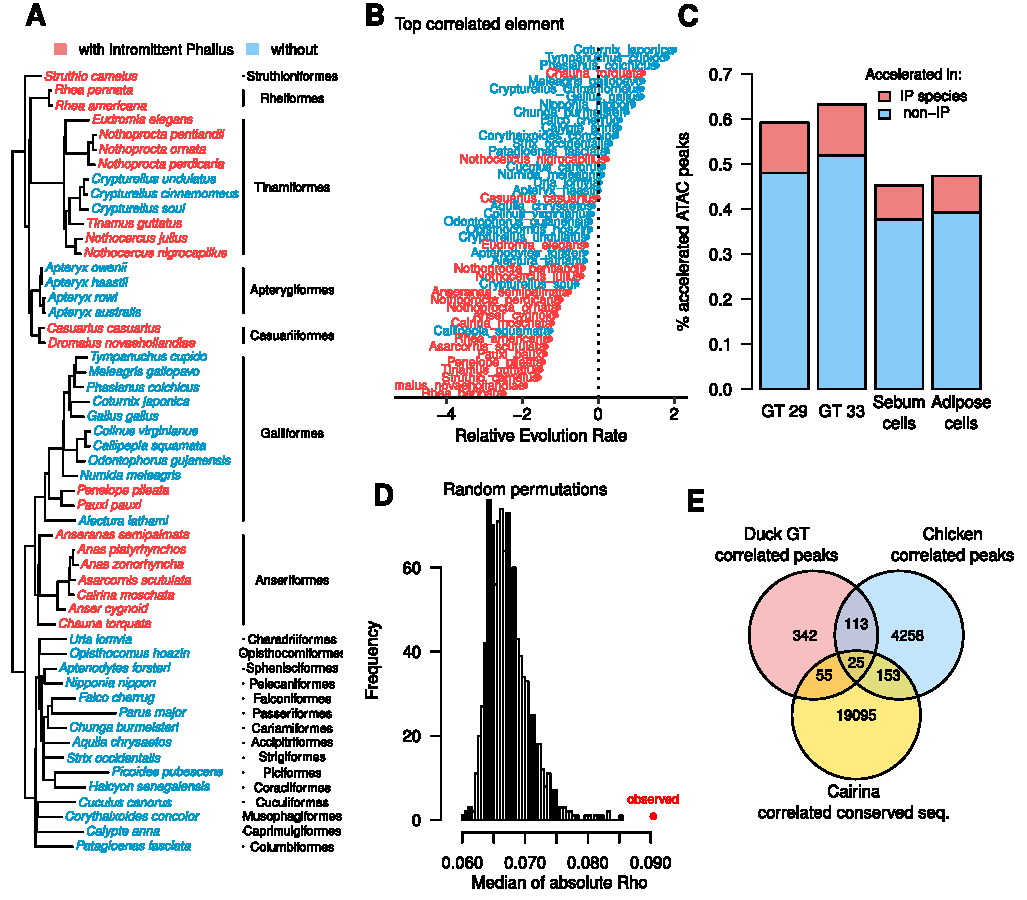
\includegraphics[width=1\textwidth, page=1] {figures/IPLOSS/Fig_evol_peaks.pdf}
    \caption[Enrichment for convergently accelerated sequences in birds that lost the intromittent phallus.]{
    \textbf{Enrichment for convergently accelerated sequences in birds that lost the intromittent phallus.}
    \textbf{A.}Species tree. Species names are coloured according to the presence (red) or absence (blue) of an intromittent phallus (IP). The Order to which the species belong is indicated. Obtained from the tree of Feng et al. 2020. 
    \textbf{B.} Example of the relative evolution rate distribution of each species obtained by RERconverge for the sequence from duck ATAC data that is the most correlated with the presence of the phallus (ref RER). Species with IP are associated with lower relative evolution rates than species without IP for this sequence. (R2=X; FDR=Y). 
    \textbf{C.} Proportion of sequences significantly correlated with the presence of IP among ATAC data from duck samples. A greater proportion of these sequences show a higher relative evolution rate in species without IP (blue) than in species with IP (red) within all samples (test; pval). The proportions of correlated sequences are significantly greater in the GT samples than in others (test; pval). 
    \textbf{D.} Distribution of the median correlation coefficients between the relative evolution rate of sequences from duck ATAC data and the presence of the phallus based on 1000 random permutations of the phenotype in the phylogeny. The observed value for the actual phenotype distribution (A.) is shown in red. 
    \textbf{E.} Overlap of homologous sequences correlated with the presence of IP depending on whether they are from duck ATAC data (red), chicken ATAC data (blue) or Cairinia moschata sequences conserved in species with PI (yellow).    \\
    }
    \label{fig:IPLOSS-fig4}
\end{figure} 

\subsection{Inference of regulatory function}

\begin{figure}[h]
    \centering
    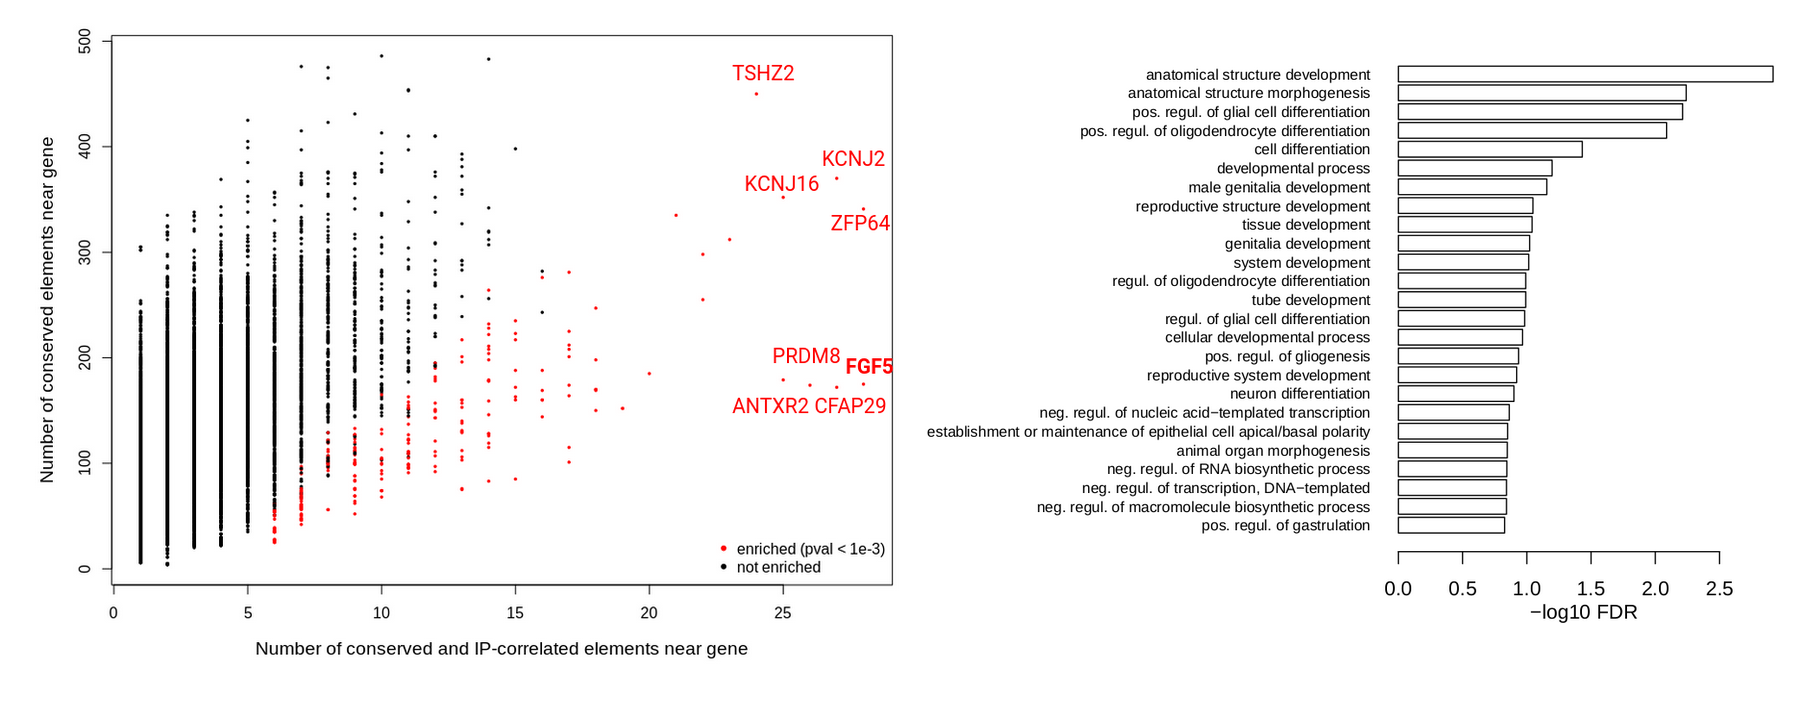
\includegraphics[width=1\textwidth, page=1] {figures/IPLOSS/Fig_enrich.png}
    \caption[Detection of genes associated with convergently accelerated sequences in no-IP species.]{
    \textbf{Detection of genes associated with convergently accelerated sequences in no-IP species.}
     \textbf{A.}  Enrichment of convergently accelerated sequences in the vicinity of genes. Each point is a gene represented by the total number of sequences and the number of accelerated sequences in its neighborhood. Colored points are genes with excess convergently accelerated sequences based on a permutation test (5\% FDR). Only genes associated with at least one accelerated sequence are plotted. 
     \textbf{B.} Ontological enrichment of genes associated with convergently accelerated sequences from duck ATAC data. Only the 25 most enriched terms are shown ordered by FDR value.
    \\
    }
    \label{fig:IPLOSS-fig5}
\end{figure} 

\section{Discussion}

\section{Methods}